\documentclass[a4paper,11pt]{article}

% ---------------------------------------------------------------------
% Language and page layout
% ---------------------------------------------------------------------
\usepackage[utf8]{inputenc}
\usepackage[T5]{fontenc}
\usepackage[english]{babel}

\usepackage{geometry}
\geometry{
    a4paper,
    total={168mm,248mm},
    left=23mm,
    top=25mm
}
\usepackage{setspace}
\usepackage{indentfirst}

% ---------------------------------------------------------------------
% Core packages retained from the original template
% ---------------------------------------------------------------------
\usepackage{float}
\usepackage{array}
\usepackage{tabularx}
\usepackage{booktabs}
\usepackage{multirow}
\usepackage{multicol}
\usepackage{longtable}
\usepackage{lscape}
\usepackage{rotating}
\usepackage{graphicx}
\usepackage[export]{adjustbox}
\usepackage{caption}
\usepackage{subcaption}
\usepackage{tablefootnote}
\usepackage{amsmath,amssymb,amsthm,amscd}
\usepackage[table,xcdraw,dvipsnames]{xcolor}
\usepackage{tikz}
\usetikzlibrary{arrows,backgrounds,positioning}
\usepackage{pgf-pie}
\usepackage[framemethod=tikz]{mdframed}
\usepackage[normalem]{ulem}
\usepackage[makeroom]{cancel}
\usepackage{enumitem}
\usepackage{lastpage}
\usepackage{subfiles}

% ---------------------------------------------------------------------
% Hyperlinks
% ---------------------------------------------------------------------
\usepackage[unicode,breaklinks,plainpages=false,pdfpagelabels]{hyperref}
\hypersetup{
    urlcolor=black,
    linkcolor=black,
    citecolor=black,
    colorlinks=true
}

% ---------------------------------------------------------------------
% Glossary / nomenclature
% ---------------------------------------------------------------------
\usepackage{etoolbox,ragged2e}

% ---------------------------------------------------------------------
% Bibliography
% ---------------------------------------------------------------------
\usepackage[
    sorting=none,
    backend=bibtex,
    natbib=true
]{biblatex}

% Bibliography database
\addbibresource{References/refs.bib}

\makeatletter
\def\blx@maxline{77}
\makeatother

% ---------------------------------------------------------------------
% English document labels
% ---------------------------------------------------------------------
\AtBeginDocument{%
    \addtocontents{toc}{\protect\thispagestyle{empty}}%
    \renewcommand{\contentsname}{Table of Contents}%
    \renewcommand{\listtablename}{List of Tables}%
    \renewcommand{\tablename}{Table}%
    \renewcommand{\listfigurename}{List of Figures}%
    \renewcommand{\figurename}{Figure}%
}


% ---------------------------------------------------------------------
% Header / footer
% ---------------------------------------------------------------------
\usepackage{fancyhdr}
\setlength{\headheight}{40pt}
\pagestyle{fancy}

\fancyhead{}
\fancyhead[L]{
 \begin{tabular}{rl}
    \begin{picture}(25,15)(0,0)
        \put(0,-8){
\includegraphics[width=8mm]{Images/hcmut.png}}
    \end{picture}
    &
    \begin{tabular}{l}
        \textbf{\ttfamily VIETNAM NATIONAL UNIVERSITY HO CHI MINH CITY}\\
        \textbf{\ttfamily HO CHI MINH CITY UNIVERSITY OF TECHNOLOGY}
    \end{tabular}
 \end{tabular}
}
\fancyhead[R]{}

\fancyfoot{}
\fancyfoot[L]{%
    \scriptsize\ttfamily
    Advanced Agentic Artificial Intelligence
}
\fancyfoot[R]{%
    \scriptsize\ttfamily
    Page {\thepage}/\pageref{LastPage}
}

\renewcommand{\headrulewidth}{0.3pt}
\renewcommand{\footrulewidth}{0.3pt}

% ---------------------------------------------------------------------
% Float spacing and captions
% ---------------------------------------------------------------------
\sloppy
\everymath{\color{black}}

\captionsetup[figure]{
    labelfont={small,bf},
    textfont={small},
    belowskip=0pt,
    aboveskip=6pt
}

\captionsetup[table]{
    labelfont={small,bf},
    textfont={small},
    belowskip=-1pt,
    aboveskip=7pt
}

\setlength{\floatsep}{5pt plus 2pt minus 2pt}
\setlength{\textfloatsep}{5pt plus 2pt minus 2pt}
\setlength{\intextsep}{10pt plus 2pt minus 2pt}

% ---------------------------------------------------------------------
% Dynamic English month name without extra packages
% ---------------------------------------------------------------------
\newcommand{\EnglishMonth}{%
    \ifcase\month
    \or January%
    \or February%
    \or March%
    \or April%
    \or May%
    \or June%
    \or July%
    \or August%
    \or September%
    \or October%
    \or November%
    \or December%
    \fi
}

\begin{document}
\hypersetup{pageanchor=false}

% =====================================================================
% TITLE PAGE
% =====================================================================
\begin{titlepage}

\begin{center}
    \color{black}
    \textbf{VIETNAM NATIONAL UNIVERSITY HO CHI MINH CITY}\\
    \textbf{HO CHI MINH CITY UNIVERSITY OF TECHNOLOGY}\\
    \textbf{FACULTY OF COMPUTER SCIENCE AND ENGINEERING}
\end{center}

\vspace{1cm}

\begin{figure}[h!]
    \centering
    
\includegraphics[width=4cm]{Images/hcmut.png}
\end{figure}

\vspace{1cm}

\begin{center}

    % Course title
    \textbf{\Large ADVANCED AGENTIC ARTIFICIAL INTELLIGENCE}\\

    \rule{0.8\textwidth}{0.4pt}\\[16pt]

    % Project title
    \parbox{0.88\textwidth}{
        \centering
        \textbf{\Huge D1 Proposal}\\[7pt]
        \textbf{\Large A Local, Evidence-Grounded}\\[2pt]
        \textbf{\Large Vietnamese Legal Assistant}
    }\\[16pt]

    \rule{0.8\textwidth}{0.4pt}

\end{center}

\vspace{0.6cm}

\begin{table}[h]
\hspace{1.7cm}
\begin{tabular}{rrl}

    & \textbf{Supervisor:} &
    \textbf{Lê Xuân Bách} \\

    \\[-2pt]

    & \textbf{Group:} &
    8, Theme 9, Application Track \\

    \\[3pt]

    & \textbf{Students:} &
    Lê Trí Quyền (Leader), 2470740 \\

    & &
    Võ Phạm Tuấn Dũng, 2570015 \\

    & &
    Nguyễn Hoàng Phong, 2570477 \\



\end{tabular}
\end{table}

\vfill

\begin{center}
    {\footnotesize
    HO CHI MINH CITY, \MakeUppercase{\EnglishMonth} \the\year
    }
\end{center}

\end{titlepage}

% =====================================================================
% FRONT MATTER
% =====================================================================
\clearpage
\hypersetup{pageanchor=true}

% =====================================================================
% MAIN CONTENT
% =====================================================================
\pagenumbering{arabic}
% =====================================================================
% chap1.tex -- D1 proposal body, LuatCheck (Application Track)
% [[...]] marks a value the team must fill in before submission.
% =====================================================================

\newcommand{\TODO}[1]{\textbf{[[#1]]}}
\newcommand{\hdr}[1]{\vspace{2pt}\noindent\textbf{#1}}

\section{Snapshot and Topic-Quality Self-Assessment}

{\small
\noindent
\begin{tabularx}{\textwidth}{@{} >{\raggedright\arraybackslash}p{2.3cm} X @{}}
\toprule
\textbf{Track / Title} & Application Track, Theme 9. \textit{LuatCheck: A Local, Evidence-Grounded Vietnamese Legal Assistant} \\
\textbf{Group 8} &
Lê Trí Quyền (Leader), retrieval and serving: ingestion, BM25 + dense index, RRF, reranking, local deployment.
Nguyễn Hoàng Phong, system and security: tool layer, UI, audit log, persistent store, fault and injection harness.
Võ Phạm Tuấn Dũng, agent and evaluation: control loop, structured output, evidence verifier, evaluation harness and analysis. \\
\textbf{Problem} & Public legal chatbots send sensitive user data outside the organization and can produce plausible but unsupported legal claims. LuatCheck targets privacy-sensitive Vietnamese legal QA with claim-level evidence verification, an explicit refusal path, and controlled tool use. \\
\textbf{Users} & Vietnamese non-lawyers (employees, small-business owners, SME administrative and HR staff) who need an understandable answer plus the provision it rests on. \\
\bottomrule
\end{tabularx}
}

\hdr{Topic-quality gate.}
\textbf{Novel:} each existing option fails on a different axis. A public assistant sends the question out of the organization, a legal portal cannot answer one, and a generic RAG chatbot cites without checking. Combining local deployment, a per-claim evidence check and a refusal path is our own choice; no tool we could simply configure offers it.
\textbf{Non-trivial:} the difficulty sits in making a 4B model behave inside the loop. It must choose among five actions under a fixed schema, recover from a failed evidence check, and stay inside a five-call budget. We expect it to fail often enough to be worth measuring, and the trade-off we measure is that verification and refusal buy grounding at the cost of coverage and latency.
\textbf{Meaningful:} deployed legal-AI tools still mis-cite in measured studies \citep{magesh2025hallucination}, while the questions users ask carry employment and identity data now regulated in Vietnam \citep{vietnam2025pdpl,decree3562025}.
\textbf{Feasible:} no model training; evaluation builds on the public VLQA Vietnamese legal QA dataset \citep{vlqa2025}; the control loop reuses one member's prior work on refusal in small tool-calling models; and we scope the build to the requirement floor, deferring the reranker and semantic verifier as optional ablations (Sec.~\ref{sec:plan}).

\section{Related Systems and Usage Scenarios}

\hdr{Why existing tools fall short.}
General assistants (ChatGPT, Gemini) answer fluently but guarantee nothing about whether a cited article exists in force, and the question itself leaves the organization. Vietnamese legal portals (thuvienphapluat.vn, vanban.chinhphu.vn) hold authoritative text but are keyword lookup: the user must already know which document to open. Commercial legal-AI research tools have been measured to still hallucinate or mis-support citations \citep{magesh2025hallucination}. Generic RAG chatbots retrieve once and generate, with no decision to search again, clarify, or refuse, and no claim-level check.

\hdr{Related work.}
RAG supplies the retrieval-grounding pattern \citep{lewis2020rag} and ReAct the interleaving of reasoning with tool use when the next action depends on intermediate evidence \citep{yao2023react}. ALCE formalizes citation-grounded generation metrics \citep{gao2023alce}; evidence that models cannot reliably self-correct without external grounding motivates checking against the retrieved store rather than asking the model to re-check itself \citep{huang2024selfcorrect}. Indirect prompt injection and tool-mediated attacks motivate strict separation of untrusted data from control flow \citep{greshake2023indirect,debenedetti2024agentdojo}. Reported agent numbers are often not reproducible and ignore cost \citep{kapoor2025agentsmatter}, so we report cost and variance beside every success metric. We keep that retrieval-grounding pattern and control loop, and add what they leave open: a failed evidence check becomes an event the loop acts on, by repairing or by refusing.

\enlargethispage{2\baselineskip}
\hdr{AT1: usage scenarios.}
(1)~An employee checks termination notice rights and receives the exact supporting provision.
(2)~SME HR staff ask a sensitive employment question without uploading the contract to a public chatbot.
(3)~\emph{Adversarial or careless:} a user pastes an untrusted document carrying an injected instruction, or asks how to evade a legal obligation, testing whether the security boundary and the refusal path hold.
We run an informal walkthrough of these scenarios with a practising SME HR contact in W5 and report it in D2.

\section{Architecture and Agentic Axes}

\begin{figure}[H]
\centering
\scalebox{0.88}{
\begin{tikzpicture}[
    node distance=0.26cm,
    every node/.style={font=\scriptsize},
    block/.style={rectangle,draw=black,rounded corners=2pt,align=center,text width=12.0cm,minimum height=0.46cm,inner sep=3pt},
    check/.style={rectangle,draw=black,dashed,rounded corners=2pt,align=center,text width=12.0cm,minimum height=0.52cm,inner sep=3pt},
    arrow/.style={->,>=stealth,thick}
]
\node[block] (input) {\textbf{User Input}: question + optional pasted document};
\node[block, below=of input] (guard) {\textbf{Input Guard}: scope/evasion check; pasted and retrieved text tagged \textbf{untrusted data}};
\node[block, below=of guard] (agent) {\textbf{Budgeted ReAct Loop}: SLM selects \texttt{search\_law}, \texttt{get\_article}, \texttt{answer}, \texttt{clarify}, or \texttt{refuse}; $\leq$5 tool calls, $\leq$2 repairs};
\node[block, below=of agent] (retrieval) {\textbf{Retrieval}: BM25 + dense $\rightarrow$ RRF $\rightarrow$ trusted article store (reranker: optional ablation)};
\node[check, below=of retrieval] (verify) {\textbf{Evidence Verification}: L1 (always): cited ID exists and was retrieved, and the claim's span is supported; L2 (optional): semantic entailment check};
\node[block, below=of verify] (decision) {\textbf{Decision}: pass $\rightarrow$ answer + citations; repair budget left $\rightarrow$ loop; repeated failure $\rightarrow$ refuse};
\node[block, below=of decision] (action) {\textbf{Guarded Action}: proposed \texttt{send\_summary} $\rightarrow$ human confirmation $\rightarrow$ execute + audit log};
\draw[arrow] (input) -- (guard);
\draw[arrow] (guard) -- (agent);
\draw[arrow] (agent) -- (retrieval);
\draw[arrow] (retrieval) -- (verify);
\draw[arrow] (verify) -- (decision);
\draw[arrow] (decision) -- (action);
\draw[arrow] (decision.east) -- ++(0.5,0) |- node[pos=0.22,right,font=\tiny]{targeted repair} (agent.east);
\end{tikzpicture}}
\caption{LuatCheck control loop. The dashed box is the deterministic verification step; the arrow returning to the loop is the repair path.}
\label{fig:d1-architecture}
\end{figure}

\vspace{-8pt}
{\small
\noindent
\begin{tabularx}{\textwidth}{@{} >{\raggedright\arraybackslash}p{2.2cm} X @{}}
\toprule
\textbf{Element} & \textbf{Design} \\
\midrule
Orchestration & Model-controlled ReAct-style loop; fixed tool and repair budgets; terminal states are answer / clarify / refuse. The action space is small and schema-constrained: agency is spent only where a fixed workflow cannot decide \citep{anthropic2024agents}. \\
Tools, permissions & \texttt{search\_law}, \texttt{get\_article}: read-only. \texttt{save\_case}: reversible write. \texttt{send\_summary}: irreversible write, executable only after explicit human confirmation. Tools are defined by JSON schemas kept MCP-compatible, so the layer can be exposed as an MCP server in D2 without changing the agent. \\
Memory (R3) & \emph{Short-term:} case ledger holding known facts, issued searches, retrieved article IDs, and the remaining budget. \emph{Long-term episodic store (R3):} SQLite. \emph{Write policy:} written only on a terminal state that passed L1 and L2, recording the normalized question, article IDs, answer, citations, verifier verdict, index version, and timestamp. A refused or unverified outcome is never written, and neither are the user's raw personal details. \emph{Retrieval policy:} lookup by embedding similarity of the question above a tuned threshold, and only when the index version matches; a hit is re-validated by L1 before reuse and the store is invalidated on index rebuild. \\
\textbf{Axis 1} & \textbf{Planning / search:} adaptive query reformulation and multi-step retrieval under budget. \\
\textbf{Axis 2} & \textbf{Reflection / verification:} L1 checks that each cited ID exists and was retrieved, then scores each generated sentence against its cited provision by sentence-embedding similarity, and we calibrate the accept threshold on the audit set of Sec.~4 and report its false-refusal rate. Failure triggers targeted repair; repeated failure produces a refusal. A semantic entailment layer (L2) is the optional ablation on top. \\
\textbf{Axis 3} & \textbf{Guardrails:} untrusted-data isolation, permissioned tools, hard budgets, controlled egress, audit logging. \\
\bottomrule
\end{tabularx}
}

\hdr{Robustness (AT2).}
Model output is schema-validated; one re-ask carrying the validator error is allowed, after which the loop falls back deterministically to \texttt{clarify} or \texttt{refuse}, never to an unchecked free-text answer. Each tool has a timeout and a bounded retry with backoff, counted against the tool budget. \texttt{send\_summary} is non-idempotent and carries an idempotency key over (case id, content hash); a repeat with the same key is suppressed and logged. If the dense index is unavailable the system degrades to BM25-only and labels the answer as degraded.

\enlargethispage{2\baselineskip}
\hdr{Deployment and operational envelope (AT3).}
The product is defined by the trust boundary rather than by one machine: all inference runs on hardware the organization controls, whether a developer workstation, an organization server, or a university GPU, and no user text leaves that boundary. Stack: Qwen3-4B for development and Qwen3-8B for evaluation via Ollama on a single consumer GPU (target $\geq$16\,GB VRAM), with a 4-bit quantized CPU configuration as the degraded floor; BM25 + Qdrant with RRF, SQLite, Streamlit. Compute cost and p50/p95 latency are reported per task and per configuration; the design targets single-user interactive use, and the scale limit (the indexed provision count, and the concurrent-session ceiling at which p95 latency exceeds 60\,s) is measured in W10 and stated in D3.

\section{Evaluation Plan}

{\small
\noindent
\begin{tabularx}{\textwidth}{@{} >{\raggedright\arraybackslash}p{2.3cm} X @{}}
\toprule
\textbf{Item} & \textbf{Plan} \\
\midrule
Task sets & Retrieval: 200 held-out query$\rightarrow$article pairs from VLQA. End-to-end: 20 tasks, namely 10 single-provision tasks derived from VLQA gold query$\rightarrow$article pairs plus 10 that we write by hand (5 synthesis, 3 unanswerable, 2 adversarial). Each task carries a user profile so clarification can be scored automatically. \\
Metrics & Retrieval: Recall@5, Recall@20, MRR. End-to-end: Unsupported-Sentence Rate~$\downarrow$, answer coverage~$\uparrow$, citation precision/recall, refusal correctness, attack-success rate, p50/p95 latency, compute cost per task. \\
Configurations & Retrieval: dense-only vs.\ hybrid + RRF (reranking added as a third point only if capacity allows). End-to-end, three configurations: local SLM, verification OFF; local SLM, verification ON (L1 + span support), the pair that isolates the claimed mechanism; and a larger self-hosted open model (Qwen3-32B via vLLM), verification ON, which bounds how much the local-deployability constraint costs in quality. A fourth configuration adding the semantic entailment layer is run only if the schedule permits. \\
Verifier audit & We label 30 (claim, provision) pairs sampled from those runs, and measure the support check's accuracy and the false-refusal rate. \\
Seeds & Seeds 42, 123, 2026 where the backend supports deterministic seeding, otherwise three independent runs at identical generation settings. We report means with variance, and claim no difference that lies within one standard error. \\
Error analysis & We categorize every failure as retrieval miss, wrong provision, unsupported claim, over-refusal, budget exhausted, or parse failure, with counts and an explanation per category. \\
Offline test & We run at least one full evaluation with networking disabled; any hidden Internet dependency fails the test. \\
\bottomrule
\end{tabularx}
}

\hdr{Model and budget.}
Every model is open-weight and self-hosted (Qwen3-4B for development, 8B for the two main configurations, 32B as the comparator), so planned API spend is zero. The cost is compute: 20 tasks $\times$ 3 seeds $\times$ 3 configurations gives 180 runs at $\leq$8 calls each, estimated with indexing and pilots at under 20 GPU-hours, the 32B comparator running on a university or organization GPU. Per course policy no run executes without token and wall-clock logging, and we report actual compute use in D3.

\section{Threat Model v0}

\noindent\textbf{Assets:} answer correctness, user data, the audit trail, egress points.
\textbf{Entry points:} the user question, a pasted document, retrieved article text, tool outputs, and the payload of a confirmed \texttt{send\_summary}, which is the system's only egress.
\textbf{Attacker:} can craft arbitrary queries and pasted documents and can plant text in retrieved content, but cannot modify the trusted legal store or the code.

\vspace{2pt}
{\small
\noindent
\begin{tabularx}{\textwidth}{@{} >{\raggedright\arraybackslash}p{3.0cm} X @{}}
\toprule
\textbf{Threat class} & \textbf{Primary defense / test} \\
\midrule
Direct and indirect prompt injection & Pasted and retrieved content is tagged untrusted and cannot alter control policy or tool permissions; exercised by the attack suite below. \\
Fabricated or unsupported citation & Deterministic ID and retrieval-membership check (L1), then claim-evidence verification against the trusted store (L2). \\
Unauthorized write or data egress & Read-only by default; human confirmation for irreversible actions; inference endpoints not changeable by the model at runtime; every \texttt{send\_summary} payload is logged before it leaves. \\
Resource and budget abuse & Hard caps on tool calls and repair rounds; predefined timeout and retry behaviour. \\
\bottomrule
\end{tabularx}
}

\enlargethispage{2\baselineskip}
\hdr{Attack suite (R6, $\geq$10 cases).}
Four direct cases in the user turn (instruction override, role-play, system-prompt exfiltration, refusal-policy bypass); four indirect cases carried by a pasted document; and at least two indirect cases planted in the system's own retrieved content via a poisoned test shard of the index. We report utility and attack-success rate separately, so refusing everything scores no better \citep{debenedetti2024agentdojo}.

\section{Work Plan, Risks, and AI-Use Statement}
\label{sec:plan}

{\small
\noindent
\begin{tabularx}{\textwidth}{@{} p{1.4cm} X @{}}
\toprule
\textbf{Week} & \textbf{Outcome (owner)} \\
\midrule
W3 & Interface contract frozen: tool JSON schemas, retrieval API, trace and log format; from here the three workstreams are independent (all). \\
W4--W5 & Corpus indexed, BM25 + dense + RRF running with first Recall@k (Quyền); budgeted loop with schema-validated output and L1 check (Dũng); UI, permissioned tool layer, audit log, SQLite store (Phong). \\
W6 & Span-support check and targeted repair; harness runs end-to-end on 10 tasks (Dũng, Quyền); guarded \texttt{send\_summary} with confirmation and idempotency key, first injection cases (Phong). \\
W7 (D2) & Checkpoint: live demo, retrieval metrics, $\geq$10 end-to-end tasks, threat model v1, first injection results (all). \\
W8--W9 & Full 20-task set, fault injection, degraded mode, user walkthrough write-up (Quyền, Phong); 3 configurations $\times$ 3 seeds, verifier audit (Dũng). \\
W10--W11 & Complete attack suite, error analysis, latency and cost measurement, fully offline run, hardening, one-command reproduction (all); reranking and the semantic entailment layer added here as extra ablation points if capacity allows. \\
W12 & D3 v1 and D4 tagged; Round 1 defense with live demo and recorded video (all). \\
\bottomrule
\end{tabularx}
}

\vspace{3pt}
{\small
\noindent
\begin{tabularx}{\textwidth}{@{} >{\raggedright\arraybackslash}p{3.2cm} X @{}}
\toprule
\textbf{Risk} & \textbf{Fallback scope} \\
\midrule
Part-time team, two members new to agentic AI & The build is scoped to the R1--R9 floor. Only one workstream is agent-specific; retrieval, UI, storage and the fault/injection harness are conventional engineering. The W3 interface contract keeps the tracks independent, and each member owns a component that appears in the evaluation. \\
No local GPU is available & The privacy claim needs organization-controlled inference: fall back to a 4-bit quantized 4B on a developer machine, then to an organization or university GPU. All three are permitted by the course compute policy, and only the latency figures change. \\
4B controller is unreliable & Move to 8B, then to the 32B configuration if needed; keep schema-constrained output and strict budgets throughout. \\
VLQA lacks article-level gold labels & Fall back to hand-authoring all 20 end-to-end tasks and building the retrieval set from a smaller sample; verified in W3 before the build starts. \\
Support check is too coarse & Deterministic citation validation is the floor and is never removed; the audit quantifies how much the span check adds, and the semantic layer is reported as a measured ablation. \\
Schedule slips & We cut in this order: the optional reranker and semantic-entailment ablations, then the verifier audit size, then the 32B comparator configuration. Preserved to the end: control loop, hybrid retrieval, L1 + span verification, long-term store, guardrails, 20 tasks with one ablation, security analysis. \\
\bottomrule
\end{tabularx}
}

\hdr{AI-use statement.}
Claude and GitHub Copilot are used for drafting, code scaffolding, and literature screening. The team manually verifies every cited source, legal claim, and design decision; all quantitative results in later deliverables come from the team's own logged runs.


% =====================================================================
% REFERENCES
% =====================================================================
\clearpage

\printbibliography[
    title={References},
    heading=bibintoc
]
\thispagestyle{fancy}

\end{document}
